\documentclass{lecturenotes}

\renewcommand{\vecka}{4}
\newcommand{\tema}{Aritmetik, Logik \& Datastrukturer}

\setbeamertemplate{footline}[frame number]
\title[Föreläsningsanteckningar EDA016, 2015]{EDA016 Programmeringsteknik för D}
\subtitle{Läsvecka \vecka: \tema}
\author{Björn Regnell}
\institute{Datavetenskap, LTH}
\date{Lp1-2, HT 2015}
 
\begin{document}

\frame{\titlepage}
\setnextsection{\vecka}
\section[Vecka \vecka: \tema]{\tema}
\frame{\tableofcontents}

%%%%%%%%%%%%%%%%%%%%%%%%%%%%%%%%%%%%%%

\subsection{Att göra denna vecka}
\frame{\frametitle{Att göra i Vecka \vecka: Förstå aritmetiska och logiska uttryck, använda klasser mha klass-specifikationer}
\begin{enumerate}
\item Läs följande kapitel i kursboken:\\ 6.1--6.4, 6.8--6.9,  7.1--7.7, 7.10--7.11, 7.13\\ 
Begrepp: heltalsdivision med rest,  implicit och explicit typkonvertering, aritmetiska och logiska uttryck, De Morgans lagar, oföränderlighet
\item Gör övning 4: Aritmetik, Logik
\item Träffas i samarbetsgrupper och hjälp varandra förstå 
\item Gör Lab 3: använda färdigskrivna klasser, kvadrat
\end{enumerate}
}


\subsection{Aritmetik}
\begin{Slide}{Primitiva datatyper i Java}
\begin{center}
\begin{tabular}{lp{6cm}}
Typ & Betydelse \\ \midrule
\Key{byte}, \Key{short}, \Key{int}, \Key{long} & heltal \\
\Key{float}, \Key{double} & reellt tal (tal med decimaldel) \\
\Key{boolean} & logiskt värde (sant eller falskt) \\
\Key{char} & tecken, till exempel bokstav, siffra, specialtecken \\
\end{tabular} 
\end{center}

\texttt{String} liknar vanliga klasser men har \href{https://docs.oracle.com/javase/specs/jls/se8/html/jls-4.html#jls-4.3.3}{speciellt stöd i språket}. Mer om detta nästa vecka. 
\end{Slide}

\begin{Slide}{Numeriska typernas storlek samt min- och max-värden}  
\begin{center}
\begin{tabular}{cccc}
Typ&	Bitar&	Min&	Max\\
\hline
\Key{byte}	&$8$	&$-128$&	$+127$\\
\Key{short}	&$16$	&$-32~768$	&$+32~767$\\
\Key{char}	&$16$	&$0$&	$65~535$\\
\Key{int}	&$32$	&$-2~147~483~648$&	$+2~147~483~647$\\
\Key{long}	&$64$	&$\approx -9\cdot 10^{18}$	&$\approx +9\cdot 10^{18}$\\
\Key{float}	&$32$	&$\approx -3.4\cdot 10^{38}$	&$\approx +3.4\cdot 10^{38}$\\
\Key{double}	&$64$	&$\approx -1.8\cdot 10^{308}$	&$\approx +-1.8\cdot 10^{308}$\\
\end{tabular}
\end{center}
För detaljer se \href{https://docs.oracle.com/javase/specs/jls/se8/html/jls-4.html#jls-4.2.3}{Javas språkspecifikation} och\\ \href{https://en.wikipedia.org/wiki/Double-precision_floating-point_format}{IEEE-standarden 754}
\end{Slide}

\begin{Slide}{Konstanter för min- och max-värden}
Några exempel:
\begin{lstlisting}
short smin = Short.MIN_VALUE;   // smin = -32768

int imax = Integer.MAX_VALUE;   // imax = 2147483647

double dmin = Double.MIN_VALUE; // dmin = 4.9E-324  
                                // OBS! pyttelitet men positivt

double dmax = Double.MAX_VALUE; // dmax = 1.8E308
\end{lstlisting}

Se vidare subklasser till \href{http://docs.oracle.com/javase/7/docs/api/java/lang/Number.html}{Number}-klassen.
\end{Slide}


\begin{Slide}{Math}
Exempel på statiska bra-att-ha-metoder i klassen \href{http://docs.oracle.com/javase/8/docs/api/java/lang/Math.html}{Math}
\begin{lstlisting}[escapechar=!, frame=, backgroundcolor=]
long round(double x);             // avrundning, även float till int 
int abs(int x);                   // !$|x|$!, även double ...
double hypot(double x, double y); // !$\sqrt{x^2+y^2}$!
double sin(double x);             // !$\sin x$! även: cos, tan, asin, atan etc. 
double exp(double x);             // !$e^x$! 
double pow(double x, double y);   // !$x^y$!
double log(double x);             // !$\ln x$ !
double sqrt(double x);            // !$\sqrt{x}$ !
double toRadians(double deg);     // !$\mathit{deg} \cdot \pi / 180$!
\end{lstlisting}
\end{Slide}

\begin{Slide}{Precisionsproblem}
\footnotesize Vad skriver nedan program ut?
\lstinputlisting[language=Java, basicstyle=\ttfamily\tiny\selectfont, numberstyle=, numbers=left,]{../examples/eclipse-ws/lecture-examples/src/week04/PrecisionProblems.java}
Se mer detaljer \href{http://stackoverflow.com/questions/2944344/java-check-if-two-double-values-match-on-specific-no-of-decimal-places}{här}.
\end{Slide}

\begin{Slide}{Deklarationer av variabler}  
\begin{lstlisting}
typ namn = startvärde;
\end{lstlisting}
\begin{itemize}
\item Om startvärdet utelämnas blir lokala variabler odefinierade, attribut får implicit startvärde (0, 0.0, \ldots).
\item Om det i en klass finns flera förekomster av samma namn så gäller den ''närmaste'' deklarationen:
\begin{lstlisting}
public class A {
    private int x; // attribut
    
    public void p() {
        int x = 0; // lokal variabel i metoden p
        // alla förekomster av "x" avser här den lokala 
        // variabeln x. Om man vill komma åt attributet
        // x skriver man this.x
    }
}
\end{lstlisting}
\end{itemize}
\end{Slide}

\begin{Slide}{Implicita  \href{http://docs.oracle.com/javase/tutorial/java/nutsandbolts/datatypes.html}{startvärden} för attribut}
Om en variabel är ett attribut (field) så ges implicita startvärden när objektet konstrueras. OBS! Detta gäller \Alert{inte} för lokala variabler som måste initialiseras före första användningen.
\begin{center}
\begin{tabular}{ll}
DataType&Default Value (for fields) \\ \hline
\Key{byte} &	0 \\
\Key{short} &	0 \\
\Key{int} 	& 0 \\
\Key{long} &	0L \\
\Key{float}  &	0.0f \\
\Key{double} & 	0.0d \\
\Key{char} &	'{\textbackslash}u0000' \\
\Key{boolean} &	false \\
\texttt{String} or any object &  	\Key{null} \\

\end{tabular}
\end{center}
\end{Slide}

\begin{Slide}{Implicit och explicit konvertering mellan numeriska värden vid tilldelning}
Tilldelningssats:
\begin{lstlisting}
variabel = uttryck;
\end{lstlisting}
\begin{itemize}
\item Variabel och uttryck ska ha \Emph{samma eller kompatibel} typ.
\item Om variabeln är ''större'' än uttryckets värde konverteras det nya värdet automatiskt till variabelns typ.
\item Om variabeln är ''mindre'' måste man konvertera explicit:
\begin{lstlisting}
int i = 100;
double d = 314.61;
short s = (short) i; // värdet av i konverteras  
                     // till short
i = (int) d;         // värdet av d konverteras 
                     // till int, 314.61 -> 314
\end{lstlisting}
\end{itemize}
\end{Slide}


\begin{Slide}{Några aritmetriska uttryck}
Heltalsuttryck:
\begin{lstlisting}[numberstyle=, numbers=left,]
int a = 0;
int b = 12;
int c = 20;
a = 2 * (b + c) + 4; // a = 68
b = a / 10;          // b = 6 (6.8, decimalerna stryks)
c = a % 10;          // c = 8 (68/10 = 6 + 8/10, 8 är resten)
\end{lstlisting}

Reella uttryck:
\begin{lstlisting}[numberstyle=, numbers=left,]
double x = 1.4;
double y = 1 + 2 * (x + 1); // y = 5.8
double z = x * x + y * y;   // z = 35.60
z = z / 10;                 // z = 3.56
int a = 5;
x = 1 + (double) a / 2;     // x = 3.5
\end{lstlisting}
\footnotesize Explicit typkonvertering har \Alert{högre} prioritet än de aritmetiska operatorerna!
\end{Slide}


\begin{Slide}{Var n-te gång, jämt delbart med n}
Vanligt trick: \lstinline+if (i % n == 0) { ... } +
\lstinputlisting[language=Java, basicstyle=\ttfamily\tiny\selectfont, numberstyle=, numbers=left,]{../examples/eclipse-ws/lecture-examples/src/week04/EveryNth.java}
\end{Slide}

\begin{Slide}{Förkortade tilldelningssatser}\footnotesize
Tilldelning med samma variabel både till höger \& vänster kan förkortas:
\begin{lstlisting}
x += dx;     // <=> x = x + dx
sum += term; // <=> sum = sum + term
nbr /= 10;   // <=> nbr = nbr / 10
\end{lstlisting}

Kortformer för att öka/minska med 1 (inkrementering/dekrementering):
\begin{lstlisting}
x++;         // <=> x = x + 1  <=> x += 1
x--;         // <=> x = x - 1  <=> x -= 1
\end{lstlisting}
Postfix och prefixnotation med \texttt{++} och \verb+--+ (använd med försiktighet)
\begin{lstlisting}
int a = 10;
int x = a++; // a blir 11, x blir 10
int b = 10;
int y = ++b; // b blir 11, y blir 11
y = --b;     // b blir 10, y blir 10
y = b--;     // b blir 9,  y blir 10
\end{lstlisting}
\end{Slide}


\subsection{Summering}
\begin{Slide}{Algoritmexempel: summering 1}
Pseudo-kod för algoritmen ''Summera värden'':
\begin{lstlisting}
sum = 0;
för alla termer {
    term = "nästa term";
    sum = sum + term;
}
\end{lstlisting}

Exempel 1: läs n; för alla n tal: läs och summera; skriv ut.

\begin{lstlisting}
Scanner scan = new Scanner(System.in);
int n = scan.nextInt(); // läs antalet tal
int sum = 0;
for (int i = 0; i < n; i++) {
    int term = scan.nextInt(); // läs nästa tal
    sum = sum + term;
}
System.out.println(sum);
\end{lstlisting}
\end{Slide}

\begin{Slide}{Algoritmexempel: summering 2}
Exempel 2: läs tills negativt tal påträffas, summera.
\begin{lstlisting}
Scanner scan = new Scanner(System.in);
int sum = 0;
int nbr = scan.nextInt();
while (nbr >= 0) {
    sum = sum + nbr;
    nbr = scan.nextInt();
}
\end{lstlisting}
Exempel 3: Beräkna summan $\displaystyle\sum^{100}_{i=1}\frac{1}{i*i}$
\begin{lstlisting}
double sum = 0;
for (int i = 1; i <= 100; i++) {
    sum = sum + 1.0 / (i * i);
}
\end{lstlisting}
\end{Slide}


\subsection{Logik}

\begin{Slide}{Logiska uttryck}
Logiska uttryck kan kopplas samman med operatorerna\\ \texttt{\&\&} (''och''), \texttt{||} (''eller''), \texttt{!} (''icke''). 

\begin{lstlisting}
int a = 3;
int b = 10;
if (a > 1 && b > 1) ...     // true
if (a < 0 || a > 10) ...    // false
if (! (a > 5)) ...          // true (a <= 5)
\end{lstlisting}

Sanningstabell för logiska operatorer:
\begin{center}
\begin{tabular}{c|c|c|c|c}
\texttt{p} & \texttt{q} & \texttt{p} \verb/&&/ \texttt{q}	 & \texttt{p || q} & \texttt{! p} \\
\hline
\Key{true} & 	\Key{true}	 & \Key{true} & \Key{true} & \Key{false} \\
\Key{true}	 & \Key{false}	 & \Key{false} & 	\Key{true}	  &\\
\Key{false} & \Key{true} & \Key{false} & \Key{true} & \Key{true} \\
\Key{false} & \Key{false} & \Key{false} & 	\Key{false} & \\
\end{tabular}
\end{center}
\end{Slide}

\begin{Slide}{Negering av logiska uttryck med \href{https://en.wikipedia.org/wiki/Augustus_De_Morgan}{De Morgans} lagar}
\footnotesize
$p$ och $q$ är logiska uttryck, $\neg$ står för ''icke'', $\wedge$ för ''och'', $\vee$ för ''eller'':
\begin{eqnarray*}
\neg (p \wedge q) & \Longleftrightarrow & (\neg p) \vee (\neg q)\\
\neg (p \vee q) & \Longleftrightarrow & (\neg p) \wedge (\neg q)\\
\end{eqnarray*}

\vspace{-5mm}
I vanligt språk:
\begin{itemize}
\item Om uttrycket består av deluttryck sammanbundna med \texttt{\&\&} eller \texttt{||}\index{"|"|@\texttt{"|"|}}, ändra alla \texttt{\&\&} till \texttt{||} och omvänt.
\item Negera alla ingående deluttryck. En relation negeras genom att man byter \texttt{==} mot \texttt{!=}, \texttt{<} mot \texttt{>=}, etc.
\end{itemize}

Exempel:

\begin{lstlisting}[escapechar=@]
! (a < b || (a == 1 && b == 1))             @$\iff$@
! (a < b) && ! (a == 1 && b == 1)           @$\iff$@
! (a < b) && (! (a == 1) || ! (b == 1))     @$\iff$@
a >= b && (a != 1 || b != 1)
\end{lstlisting}
\end{Slide}



\subsection{Datastrukturer}
\begin{Slide}{Vad är en datastruktur?}
En datastruktur:

\begin{itemize}
\item kan innehålla många element,
\item har \emph{ett} namn,
\item och man kan komma åt de enskilda elementen.
\end{itemize}

Har man många element av samma typ kan man organisera elementen på olika sätt, till exempel som listor, träd eller grafer:
\begin{center}

\includegraphics[width=8cm]{img/lista.pdf}\\
\vspace{5mm}
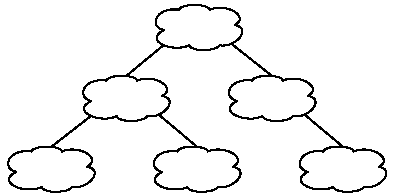
\includegraphics[width=4cm]{img/trad.pdf}
\hspace{5mm}
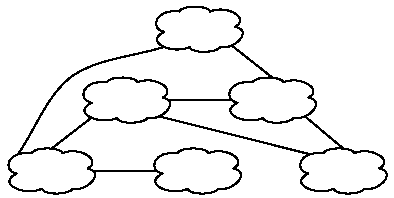
\includegraphics[width=4cm]{img/graf.pdf}
\end{center}
Mer om detta i fortsättningskursen...
\end{Slide}

\begin{Slide}{Klass som datastruktur}
\begin{itemize}
\item En enkel form av datastruktur är att kapsla in olika element som hänger i hop i en \Emph{post} \Eng{record}. \\Kallas även \Emph{tupel} \Eng{tuple}. \\ Exempel: en post med persondata innehåller fälten \textit{förnamn}, \textit{efternamn}, \textit{personnummer}
\item I många programspråk finns speciella språkkonstruktioner för detta (\texttt{record} i \href{http://www.tutorialspoint.com/pascal/pascal_records.htm}{Pascal}, \texttt{struct} i \href{https://en.wikipedia.org/wiki/Struct_\%28C_programming_language\%29}{C}, \texttt{Tuple} i \href{http://www.tutorialspoint.com/scala/scala_tuples.htm}{Scala}). 
\item I objektorienterade språk kan man använda attribut i klasser för att skapa en sådan datastruktur. En klass kan erbjuda både lagring av data i en (intern) struktur och operationer för att läsa och bearbeta data. \\ \Emph{Klasser  samlar  data och operationer på data.}
\end{itemize}
\end{Slide}

\begin{Slide}{Exempel på klass som datastruktur: Person}
\lstinputlisting[language=Java, basicstyle=\ttfamily\fontsize{5}{5.5}\selectfont, numberstyle=, numbers=left,]{../examples/eclipse-ws/lecture-examples/src/week04/Person.java}
\scriptsize För den nyfikne: läs om \href{https://en.wikipedia.org/wiki/Boilerplate_code}{boilerplate code} och \href{http://programmers.stackexchange.com/questions/30297/is-there-any-reason-to-use-plain-old-data-classes}{denna diskussion}
\end{Slide}

\subsection{Specifikationer och implementationer}

\begin{Slide}{Specifikation av klassen \texttt{BankAccount}}
\begin{ClassSpec}{BankAccount}
/** Skapar ett bankkonto med numret accntNbr och
    saldot noll */
BankAccount(int accntNbr); 

/** Tar reda på kontonumret */
int getAccntNbr();

/** Tar reda på saldot */
int getBalance();

/** Sätter in amount kronor på kontot */
void deposit(int amount);

/** Tar ut amount kronor från kontot */
void withdraw(int amount);
\end{ClassSpec}
\end{Slide}

\begin{Slide}{Implementation av klassen \texttt{BankAccount}, 1}
\begin{lstlisting}
public class BankAccount {
    private int accntNbr; // kontonummer
    private int balance;  // saldo

    /** Skapar ett bankkonto med numret accntNbr och saldot noll */
    public BankAccount(int accntNbr) {
        this.accntNbr = accntNbr;
        this.balance = 0;
    }

    /** Tar reda på kontonumret */
    public int getAccntNbr() {
        return accntNbr;
    }
\end{lstlisting}
\end{Slide}

\begin{Slide}{Implementation av klassen \texttt{BankAccount}, 2}
\begin{lstlisting}
    /** Tar reda på saldot */
    public int getBalance() {
        return balance;
    }

    /** Sätter in amount kronor på kontot */
    public void deposit(int amount) {
        balance = balance + amount;
    }
    
    /** Tar ut amount kronor från kontot */
    public void withdraw(int amount) {
        balance = balance - amount;
    }
}
\end{lstlisting}
\end{Slide}

\begin{Slide}{Bankkonto med ränta}\footnotesize
\Emph{Krav} på bankkonto med ränta:
\begin{enumerate}
\item Ränta för varje dag som pengar finns på kontot skall ackumuleras.
\item Vid årsskiftet skall räntan sättas in på kontot.
\end{enumerate}
\Emph{Design} av bankkonto-klass med ränta:
\begin{itemize}
  \item Attributet \texttt{interestRate} anger räntesatsen i procent för kontot.
  \item Den ackumulerade räntan (attributet \texttt{interest}) ökas genom anrop av metoden \texttt{computeInterest()} varje gång som saldot förändras genom insättning eller uttag.
  \item Attributet \texttt{lastInterestDay} anger numret på den dag (med början på nummer 1 för den 1 januari) då räntan senast beräknades.
  \item Metoden \texttt{Date.today()} ger numret på aktuell dag.
  \item I slutet av ett år läggs den ackumulerade räntan till saldot när någon ''utifrån'' utför operationen \texttt{newYearActions()}.
\end{itemize}
Se hela lösningen \href{https://github.com/bjornregnell/lth-eda016-2015/blob/master/lectures/examples/eclipse-ws/lecture-examples/src/week04/BankAccountWithInterest.java}{här}. (Designen är inte särskilt realistisk... Varför?)
\end{Slide} 

\begin{Slide}{Implementation \texttt{BankAccountWithInterest}, 1}
\Emph{Abstraktion}: \\Vi löser delproblemet att räkna ränta i en egen metod
\begin{Code}
public class BankAccountWithInterest {
    private int accntNbr;        // kontonummer
    private int balance;         // saldo
    private double interestRate; // räntesats i procent
    private double interest;     // ackumulerad ränta under året
    private int lastInterestDay; // dagnummer för senaste ränteberäkning

    //... konstruktor, getters/setters (visas ej)
    
    public void deposit(int amount) {
        computeInterest();
        balance = balance + amount;
    }
\end{Code}
\end{Slide} 

\begin{Slide}{Implementation \texttt{BankAccountWithInterest}, 2}
\Emph{Abstraktion}: \\Vi återanvänder lösningen på delproblemet att räkna ränta
\begin{Code}
    /** Adderar årets ränta till saldot. Ska utföras vid årsskifte */
    public void newYearActions() {
        computeInterest();
        balance = balance + (int) Math.round(interest);
        interest = 0;
        lastInterestDay = 1;
    }
    
    /** Adderar räntan sedan föregående insättning eller uttag */
    private void computeInterest() {
        interest = interest + interestRate / 100.0 *
                   (Date.today() - lastInterestDay) / 
                   360 * balance;
        lastInterestDay = Date.today();
    } 
}
\end{Code}
\end{Slide} 

\begin{Slide}{Specifikation av klassen \texttt{Square}}
\begin{ClassSpec}{Square}
/** Skapar en kvadrat med övre vänstra hörnet i x,y och med sidlängden side  */
Square(int x, int y, int side);

/** Ritar kvadraten i fönstret w */
void draw(SimpleWindow w);

/** Flyttar kvadraten avståndet dx i x-led, dy i y-led */
void move(int dx, int dy);

/** Tar reda på x-koordinaten för kvadratens läge */
int getX();

/** Tar reda på y-koordinaten för kvadratens läge */
int getY();

/** Tar reda på kvadratens area */
int getArea();
\end{ClassSpec}
Den interna representationen av kvadratens läge är \textit{inte} stipulerad av specifikationen -- det är upp till implementatören.
\end{Slide}

\begin{Slide}{Specifikation av \texttt{SimpleWindow}}
Så här ser delar av specifikationen för \texttt{SimpleWindow} ut i ankboken Appendix C, sidan 309-312.
\begin{ClassSpec}{SimpleWindow}
/** Creates a window and makes it visible. */
SimpleWindow(int width, int height, java.lang.String title);

/** Moves the pen to a new position. */
void moveTo(int x, int y)

/** Moves the pen to a new position while drawing a line. */
void lineTo(int x, int y)
\end{ClassSpec}
Specifikationerna i ankboken liknar (en enklare variant av) javadoc som genereras ur dokumentationskommentarer. Jämför med \href{http://fileadmin.cs.lth.se/cs/Education/EDA016/2015/doc/se/lth/cs/pt/window/SimpleWindow.html}{javadoc för \texttt{SimpleWindow}}
\end{Slide}

\begin{Slide}{Implementation av (delar av) Square-klassen}
\lstinputlisting[language=Java, basicstyle=\ttfamily\tiny\selectfont, numberstyle=, numbers=left,]{../examples/eclipse-ws/lecture-examples/src/week04/Square.java}
\end{Slide}

\begin{Slide}{Varför privata attribut?}
Två viktiga anledningar till att göra attribut \Key{private} och bara tillåta åtkomst av data via metoder:
\begin{enumerate}
\item I metoder kan vi \Emph{validera indata} och säkerställa så att manipuleringen blir rätt, till exempel att vi inte tillåter negativ ränta (eller ska vi tillåta det? -- ta reda på kraven...)
\item Vi kan \Emph{ändra den interna representationen} av data och alltså byta datastruktur utan att behöva ändra alla metodanrop i koden som använder vår klass.
\end{enumerate}
\footnotesize Nackdelen i Java är boilerplate (getters, setters)... Men en bra IDE kan hjälpa till att generera mallar för dessa med ett enkelt menykommando.\\ \scriptsize Vissa språk har explicit stöd för \href{https://en.wikipedia.org/wiki/Property_\%28programming\%29}{properties} med getter/setter-par (t.ex. JavaScript, C\#, Scala)  och vissa uppfyller \href {https://en.wikipedia.org/wiki/Uniform_access_principle}{uniform access principle} (t.ex. Ruby, Python, Scala) där man kan använda samma syntax oavsett om det är en metod eller ett attribut.
\end{Slide}

\begin{Slide}{Ändra den interna representationen av kvadratens läge}
Läget hos en kvadrat kan representeras av ett \texttt{Point}-objekt i stället för av koordinaterna \texttt{x} och \texttt{y}:
\begin{Code}
private Point location; // övre vänstra hörnet
private int side;       // sidlängd
\end{Code}

\begin{ClassSpec}{Point}
/** Skapar en punkt med koordinaterna x, y */
Point(int x, int y); 

/** Tar reda på x-koordinaten */
int getX();

/** Tar reda på y-koordinaten */
int getY();

/** Flyttar punkten avståndet dx i x-led, 
    dy i y-led */
void move(int dx, int dy);
\end{ClassSpec}
\end{Slide}


\Subsection{Oföränderlighet (immutability)}
\begin{Slide}{Om man kan undvika förändring blir det mycket lättare}
\begin{itemize}
\item Varje förändring av variablers värden (ändring av tillstånd) är svåra att resonera om och ger lätt upphov till buggar.
\item Vi tränar mycket på att \Alert{mutera} värden i denna kurs, men i praktiken är det ofta bra att \Alert{undvika} mutering.
\item Om man ska utnyttja flera trådar och parallell exekvering kräver föränderliga variabler \Emph{synkronisering} så att olika trådar inte förstör för varandra och svårhittade buggar uppkommer. Mer om detta i \href{http://cs.lth.se/eda040}{realtidsprogrammering}.
\end{itemize}
\end{Slide}


\begin{Slide}{Förhindra att variabler \href{https://docs.oracle.com/javase/tutorial/essential/concurrency/immutable.html}{ändras} med \texttt{\textbf{final}}}
Attributet \texttt{latinsktNamn} nedan är en \Emph{konstant}.\\ Kompilatorn hjälper oss att kolla så att vi inte råkar ändra på det vi har deklarerat som \Key{final}.
\lstinputlisting[language=Java, basicstyle=\ttfamily\tiny\selectfont, numberstyle=, numbers=left,]{../examples/terminal/final/Constant.java}
\end{Slide}

\begin{Slide}{Oföränderligt objekt}
\lstinputlisting[language=Java, basicstyle=\ttfamily\tiny\selectfont, numberstyle=, numbers=left,]{../examples/terminal/final/ImmutableObject.java}
\end{Slide}

\Subsection{Hjälpmedel på tenta: ''snabbreferens''}
\begin{Slide}{Enda hjälpmedlet på kontrollskrivning och tenta}
Ta med denna snabbreferens \Emph{på papper} vid examination: \\ 
\url{http://cs.lth.se/eda016/javaref} \\ \vspace{1em}
\Alert{Träna på att hitta i den och att använda den!} \\ \vspace{1em}
\textit{Innehåll:} satser, uttryck, deklarationer, klasser, standardklasser: Object, Math, System, Integer, String, StringBuilder, List, ArrayList, LinkedList, Random, Scanner), läsa/skriva till/från fil  
\end{Slide}

\begin{Slide}{Träna på kontrollskrivning och tenta}
\begin{itemize}
\item Det är svårt även för en van programmerare att ta tentan om man inte tränar!
\item Jag vill att \Emph{alla} tränar mycket på att programmera utan hjälpmedel och att \Emph{alla} siktar på \Alert{högsta betyg}!
\item Boka in \Alert{2h} i läsvecka 5 (nästa vecka) med din samarbetsgrupp för att \Emph{träna inför kontrollskrivning}.
\item Följ instruktionerna på kurshemsidan: \\ \href{http://cs.lth.se/eda016/examination/}{Examination $\rightarrow$ Träna inför diagnostisk kontrollskrivning}
\end{itemize}
\end{Slide}

\end{document}